\documentclass[1p]{elsarticle_modified}
%\bibliographystyle{elsarticle-num}

%\usepackage[colorlinks]{hyperref}
%\usepackage{abbrmath_seonhwa} %\Abb, \Ascr, \Acal ,\Abf, \Afrak
\usepackage{amsfonts}
\usepackage{amssymb}
\usepackage{amsmath}
\usepackage{amsthm}
\usepackage{scalefnt}
\usepackage{amsbsy}
\usepackage{kotex}
\usepackage{caption}
\usepackage{subfig}
\usepackage{color}
\usepackage{graphicx}
\usepackage{xcolor} %% white, black, red, green, blue, cyan, magenta, yellow
\usepackage{float}
\usepackage{setspace}
\usepackage{hyperref}

\usepackage{tikz}
\usetikzlibrary{arrows}

\usepackage{multirow}
\usepackage{array} % fixed length table
\usepackage{hhline}

%%%%%%%%%%%%%%%%%%%%%
\makeatletter
\renewcommand*\env@matrix[1][\arraystretch]{%
	\edef\arraystretch{#1}%
	\hskip -\arraycolsep
	\let\@ifnextchar\new@ifnextchar
	\array{*\c@MaxMatrixCols c}}
\makeatother %https://tex.stackexchange.com/questions/14071/how-can-i-increase-the-line-spacing-in-a-matrix
%%%%%%%%%%%%%%%

\usepackage[normalem]{ulem}

\newcommand{\msout}[1]{\ifmmode\text{\sout{\ensuremath{#1}}}\else\sout{#1}\fi}
%SOURCE: \msout is \stkout macro in https://tex.stackexchange.com/questions/20609/strikeout-in-math-mode

\newcommand{\cancel}[1]{
	\ifmmode
	{\color{red}\msout{#1}}
	\else
	{\color{red}\sout{#1}}
	\fi
}

\newcommand{\add}[1]{
	{\color{blue}\uwave{#1}}
}

\newcommand{\replace}[2]{
	\ifmmode
	{\color{red}\msout{#1}}{\color{blue}\uwave{#2}}
	\else
	{\color{red}\sout{#1}}{\color{blue}\uwave{#2}}
	\fi
}

\newcommand{\Sol}{\mathcal{S}} %segment
\newcommand{\D}{D} %diagram
\newcommand{\A}{\mathcal{A}} %arc


%%%%%%%%%%%%%%%%%%%%%%%%%%%%%5 test

\def\sl{\operatorname{\textup{SL}}(2,\Cbb)}
\def\psl{\operatorname{\textup{PSL}}(2,\Cbb)}
\def\quan{\mkern 1mu \triangleright \mkern 1mu}

\theoremstyle{definition}
\newtheorem{thm}{Theorem}[section]
\newtheorem{prop}[thm]{Proposition}
\newtheorem{lem}[thm]{Lemma}
\newtheorem{ques}[thm]{Question}
\newtheorem{cor}[thm]{Corollary}
\newtheorem{defn}[thm]{Definition}
\newtheorem{exam}[thm]{Example}
\newtheorem{rmk}[thm]{Remark}
\newtheorem{alg}[thm]{Algorithm}

\newcommand{\I}{\sqrt{-1}}
\begin{document}

%\begin{frontmatter}
%
%\title{Boundary parabolic representations of knots up to 8 crossings}
%
%%% Group authors per affiliation:
%\author{Yunhi Cho} 
%\address{Department of Mathematics, University of Seoul, Seoul, Korea}
%\ead{yhcho@uos.ac.kr}
%
%
%\author{Seonhwa Kim} %\fnref{s_kim}}
%\address{Center for Geometry and Physics, Institute for Basic Science, Pohang, 37673, Korea}
%\ead{ryeona17@ibs.re.kr}
%
%\author{Hyuk Kim}
%\address{Department of Mathematical Sciences, Seoul National University, Seoul 08826, Korea}
%\ead{hyukkim@snu.ac.kr}
%
%\author{Seokbeom Yoon}
%\address{Department of Mathematical Sciences, Seoul National University, Seoul, 08826,  Korea}
%\ead{sbyoon15@snu.ac.kr}
%
%\begin{abstract}
%We find all boundary parabolic representation of knots up to 8 crossings.
%
%\end{abstract}
%\begin{keyword}
%    \MSC[2010] 57M25 
%\end{keyword}
%
%\end{frontmatter}

%\linenumbers
%\tableofcontents
%
\newcommand\colored[1]{\textcolor{white}{\rule[-0.35ex]{0.8em}{1.4ex}}\kern-0.8em\color{red} #1}%
%\newcommand\colored[1]{\textcolor{white}{ #1}\kern-2.17ex	\textcolor{white}{ #1}\kern-1.81ex	\textcolor{white}{ #1}\kern-2.15ex\color{red}#1	}

{\Large $\underline{11a_{25}~(K11a_{25})}$}

\setlength{\tabcolsep}{10pt}
\renewcommand{\arraystretch}{1.6}
\vspace{1cm}\begin{tabular}{m{100pt}>{\centering\arraybackslash}m{274pt}}
\multirow{5}{120pt}{
	\centering
	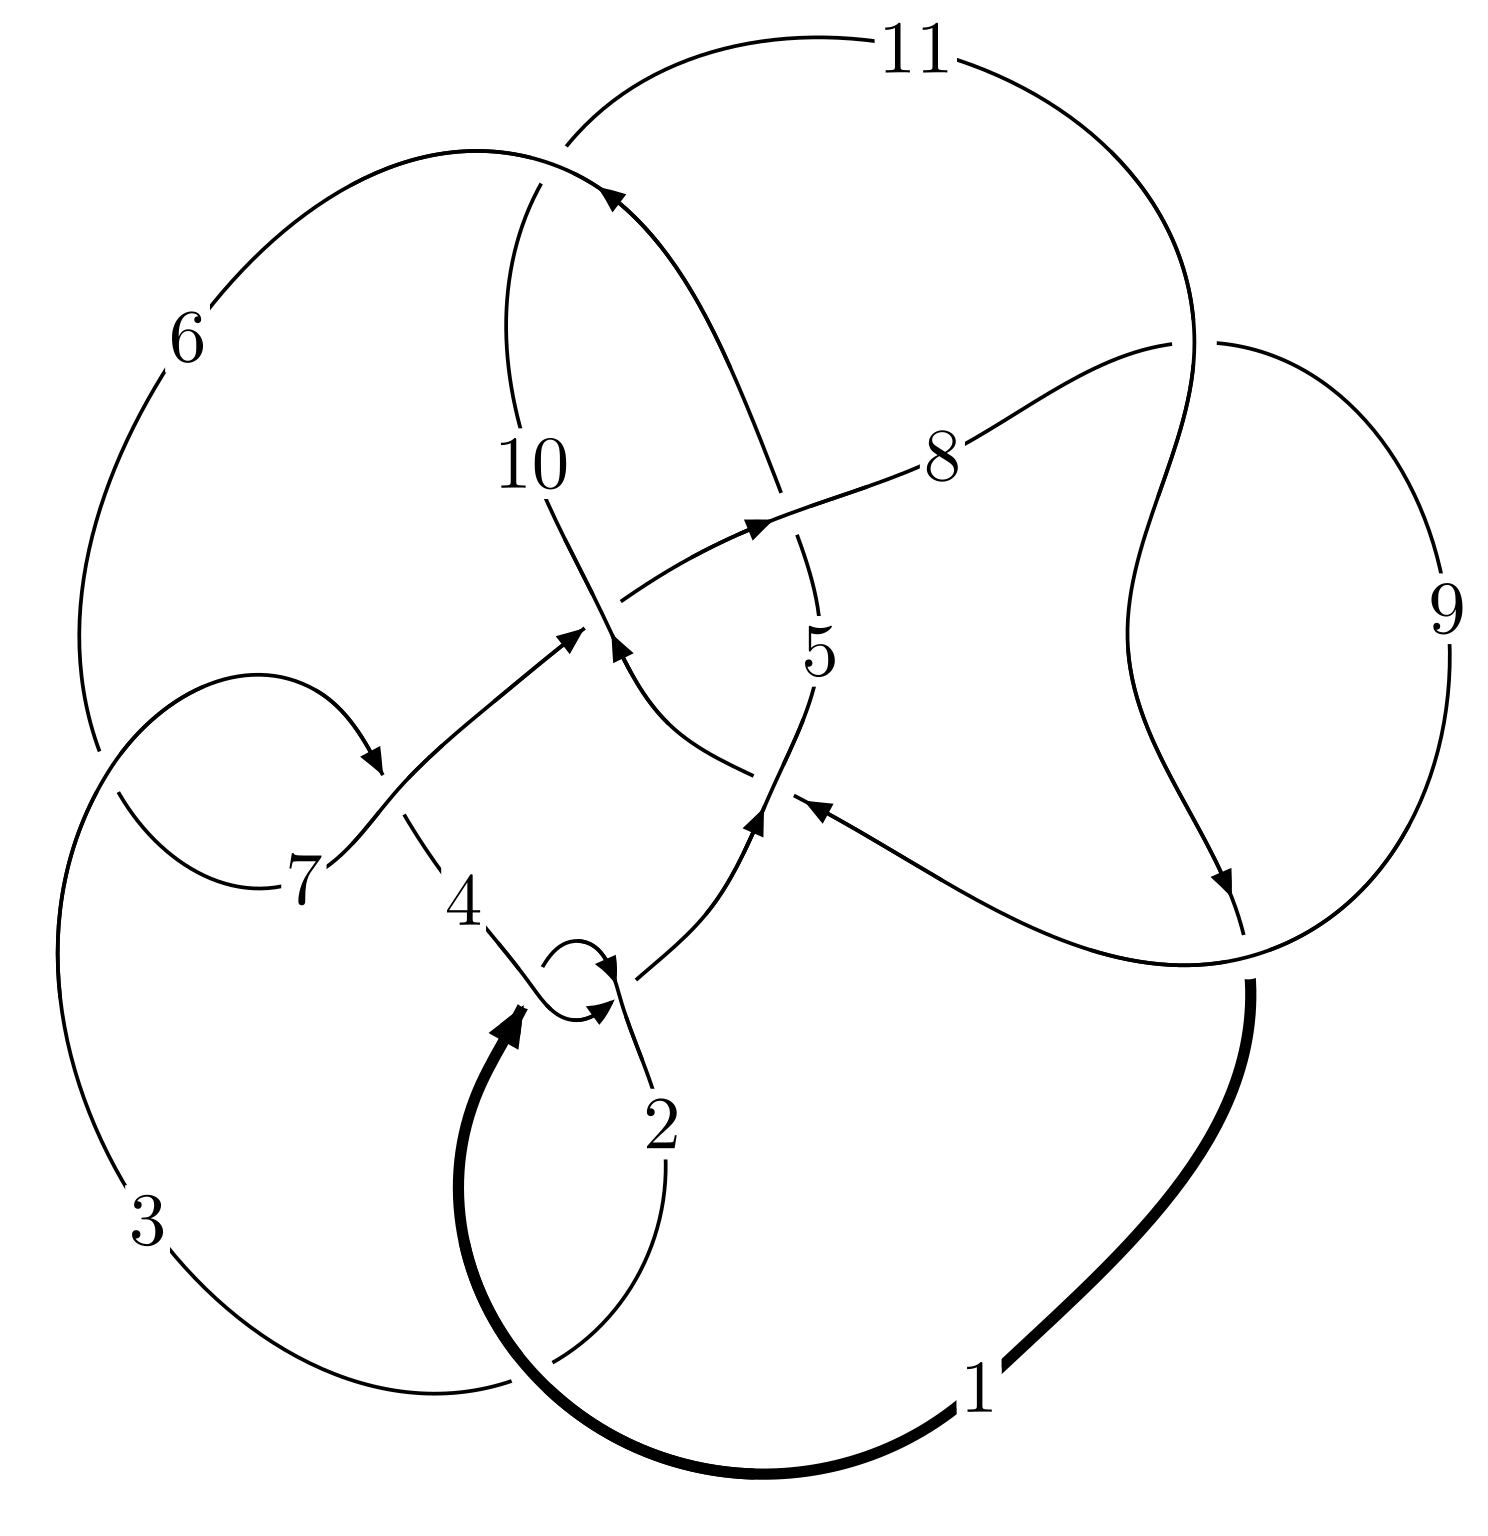
\includegraphics[width=112pt]{../../../GIT/diagram.site/Diagrams/png/274_11a_25.png}\\
\ \ \ A knot diagram\footnotemark}&
\allowdisplaybreaks
\textbf{Linearized knot diagam} \\
\cline{2-2}
 &
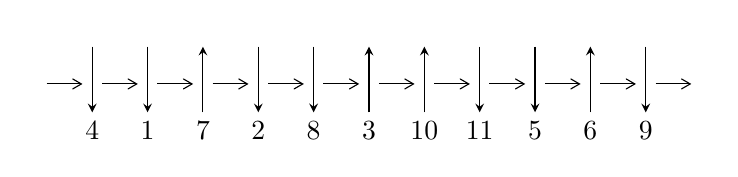
\begin{tikzpicture}[x=20pt, y=17pt]
	% nodes
	\node (C0) at (0, 0) {};
	\node (C1) at (1, 0) {};
	\node (C1U) at (1, +1) {};
	\node (C1D) at (1, -1) {4};

	\node (C2) at (2, 0) {};
	\node (C2U) at (2, +1) {};
	\node (C2D) at (2, -1) {1};

	\node (C3) at (3, 0) {};
	\node (C3U) at (3, +1) {};
	\node (C3D) at (3, -1) {7};

	\node (C4) at (4, 0) {};
	\node (C4U) at (4, +1) {};
	\node (C4D) at (4, -1) {2};

	\node (C5) at (5, 0) {};
	\node (C5U) at (5, +1) {};
	\node (C5D) at (5, -1) {8};

	\node (C6) at (6, 0) {};
	\node (C6U) at (6, +1) {};
	\node (C6D) at (6, -1) {3};

	\node (C7) at (7, 0) {};
	\node (C7U) at (7, +1) {};
	\node (C7D) at (7, -1) {10};

	\node (C8) at (8, 0) {};
	\node (C8U) at (8, +1) {};
	\node (C8D) at (8, -1) {11};

	\node (C9) at (9, 0) {};
	\node (C9U) at (9, +1) {};
	\node (C9D) at (9, -1) {5};

	\node (C10) at (10, 0) {};
	\node (C10U) at (10, +1) {};
	\node (C10D) at (10, -1) {6};

	\node (C11) at (11, 0) {};
	\node (C11U) at (11, +1) {};
	\node (C11D) at (11, -1) {9};
	\node (C12) at (12, 0) {};

	% arrows
	\draw[->,>={angle 60}]
	(C0) edge (C1) (C1) edge (C2) (C2) edge (C3) (C3) edge (C4) (C4) edge (C5) (C5) edge (C6) (C6) edge (C7) (C7) edge (C8) (C8) edge (C9) (C9) edge (C10) (C10) edge (C11) (C11) edge (C12) ;	\draw[->,>=stealth]
	(C1U) edge (C1D) (C2U) edge (C2D) (C3D) edge (C3U) (C4U) edge (C4D) (C5U) edge (C5D) (C6D) edge (C6U) (C7D) edge (C7U) (C8U) edge (C8D) (C9U) edge (C9D) (C10D) edge (C10U) (C11U) edge (C11D) ;
	\end{tikzpicture} \\
\hhline{~~} \\& 
\textbf{Solving Sequence} \\ \cline{2-2} 
 &
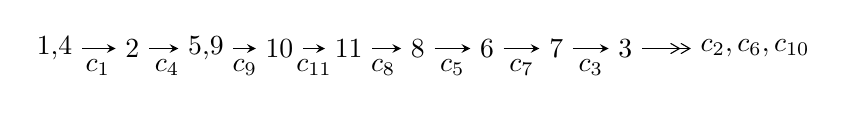
\begin{tikzpicture}[x=25pt, y=7pt]
	% node
	\node (A0) at (-1/8, 0) {1,4};
	\node (A1) at (1, 0) {2};
	\node (A2) at (33/16, 0) {5,9};
	\node (A3) at (25/8, 0) {10};
	\node (A4) at (33/8, 0) {11};
	\node (A5) at (41/8, 0) {8};
	\node (A6) at (49/8, 0) {6};
	\node (A7) at (57/8, 0) {7};
	\node (A8) at (65/8, 0) {3};
	\node (C1) at (1/2, -1) {$c_{1}$};
	\node (C2) at (3/2, -1) {$c_{4}$};
	\node (C3) at (21/8, -1) {$c_{9}$};
	\node (C4) at (29/8, -1) {$c_{11}$};
	\node (C5) at (37/8, -1) {$c_{8}$};
	\node (C6) at (45/8, -1) {$c_{5}$};
	\node (C7) at (53/8, -1) {$c_{7}$};
	\node (C8) at (61/8, -1) {$c_{3}$};
	\node (A9) at (10, 0) {$c_{2},c_{6},c_{10}$};

	% edge
	\draw[->,>=stealth]	
	(A0) edge (A1) (A1) edge (A2) (A2) edge (A3) (A3) edge (A4) (A4) edge (A5) (A5) edge (A6) (A6) edge (A7) (A7) edge (A8) ;
	\draw[->>,>={angle 60}]	
	(A8) edge (A9);
\end{tikzpicture} \\ 

\end{tabular} \\

\footnotetext{
The image of knot diagram is generated by the software ``\textbf{Draw programme}" developed by Andrew Bartholomew(\url{http://www.layer8.co.uk/maths/draw/index.htm\#Running-draw}), where we modified some parts for our purpose(\url{https://github.com/CATsTAILs/LinksPainter}).
}\phantom \\ \newline 
\centering \textbf{Ideals for irreducible components\footnotemark of $X_{\text{par}}$} 
 
\begin{align*}
I^u_{1}&=\langle 
-1.14096\times10^{69} u^{81}-5.58994\times10^{69} u^{80}+\cdots+1.56549\times10^{69} b+2.41728\times10^{69},\\
\phantom{I^u_{1}}&\phantom{= \langle  }-1.59096\times10^{68} u^{81}-1.08869\times10^{69} u^{80}+\cdots+9.78432\times10^{67} a+1.01297\times10^{69},\;u^{82}+6 u^{81}+\cdots-8 u-1\rangle \\
I^u_{2}&=\langle 
b^5- b^4-2 b^3+b^2+b+1,\;a-1,\;u-1\rangle \\
\\
\end{align*}
\raggedright * 2 irreducible components of $\dim_{\mathbb{C}}=0$, with total 87 representations.\\
\footnotetext{All coefficients of polynomials are rational numbers. But the coefficients are sometimes approximated in decimal forms when there is not enough margin.}
\newpage
\renewcommand{\arraystretch}{1}
\centering \section*{I. $I^u_{1}= \langle -1.14\times10^{69} u^{81}-5.59\times10^{69} u^{80}+\cdots+1.57\times10^{69} b+2.42\times10^{69},\;-1.59\times10^{68} u^{81}-1.09\times10^{69} u^{80}+\cdots+9.78\times10^{67} a+1.01\times10^{69},\;u^{82}+6 u^{81}+\cdots-8 u-1 \rangle$}
\flushleft \textbf{(i) Arc colorings}\\
\begin{tabular}{m{7pt} m{180pt} m{7pt} m{180pt} }
\flushright $a_{1}=$&$\begin{pmatrix}1\\0\end{pmatrix}$ \\
\flushright $a_{4}=$&$\begin{pmatrix}0\\u\end{pmatrix}$ \\
\flushright $a_{2}=$&$\begin{pmatrix}1\\u^2\end{pmatrix}$ \\
\flushright $a_{5}=$&$\begin{pmatrix}- u\\- u^3+u\end{pmatrix}$ \\
\flushright $a_{9}=$&$\begin{pmatrix}1.62603 u^{81}+11.1269 u^{80}+\cdots-32.4970 u-10.3530\\0.728817 u^{81}+3.57073 u^{80}+\cdots-2.46718 u-1.54411\end{pmatrix}$ \\
\flushright $a_{10}=$&$\begin{pmatrix}-2.60869 u^{81}-11.2390 u^{80}+\cdots-2.43637 u-5.89186\\5.06035 u^{81}+21.3826 u^{80}+\cdots-12.4229 u-2.96275\end{pmatrix}$ \\
\flushright $a_{11}=$&$\begin{pmatrix}1.50444 u^{81}+10.5800 u^{80}+\cdots-34.0990 u-11.2965\\1.80874 u^{81}+9.46187 u^{80}+\cdots-11.7179 u-3.24701\end{pmatrix}$ \\
\flushright $a_{8}=$&$\begin{pmatrix}-0.393237 u^{81}-2.05370 u^{80}+\cdots+5.46852 u+3.40029\\-2.58681 u^{81}-15.0269 u^{80}+\cdots+30.1392 u+5.36022\end{pmatrix}$ \\
\flushright $a_{6}=$&$\begin{pmatrix}3.69251 u^{81}+18.0231 u^{80}+\cdots-19.9154 u-0.624870\\-2.07099 u^{81}-5.98340 u^{80}+\cdots-5.40373 u-0.423689\end{pmatrix}$ \\
\flushright $a_{7}=$&$\begin{pmatrix}-2.73425 u^{81}-10.6085 u^{80}+\cdots-4.73671 u-3.63574\\-4.68430 u^{81}-29.2185 u^{80}+\cdots+55.5656 u+7.41855\end{pmatrix}$ \\
\flushright $a_{3}=$&$\begin{pmatrix}- u^2+1\\u^2\end{pmatrix}$\\ \flushright $a_{3}=$&$\begin{pmatrix}- u^2+1\\u^2\end{pmatrix}$\\&\end{tabular}
\flushleft \textbf{(ii) Obstruction class $= -1$}\\~\\
\flushleft \textbf{(iii) Cusp Shapes $= 11.3752 u^{81}+53.0887 u^{80}+\cdots-66.0984 u-14.2656$}\\~\\
\newpage\renewcommand{\arraystretch}{1}
\flushleft \textbf{(iv) u-Polynomials at the component}\newline \\
\begin{tabular}{m{50pt}|m{274pt}}
Crossings & \hspace{64pt}u-Polynomials at each crossing \\
\hline $$\begin{aligned}c_{1},c_{4}\end{aligned}$$&$\begin{aligned}
&u^{82}-6 u^{81}+\cdots+8 u-1
\end{aligned}$\\
\hline $$\begin{aligned}c_{2}\end{aligned}$$&$\begin{aligned}
&u^{82}+42 u^{81}+\cdots+32 u+1
\end{aligned}$\\
\hline $$\begin{aligned}c_{3},c_{6}\end{aligned}$$&$\begin{aligned}
&u^{82}- u^{81}+\cdots+160 u+32
\end{aligned}$\\
\hline $$\begin{aligned}c_{5}\end{aligned}$$&$\begin{aligned}
&u^{82}-6 u^{81}+\cdots+2 u-1
\end{aligned}$\\
\hline $$\begin{aligned}c_{7}\end{aligned}$$&$\begin{aligned}
&u^{82}+14 u^{81}+\cdots+2 u+1
\end{aligned}$\\
\hline $$\begin{aligned}c_{8},c_{11}\end{aligned}$$&$\begin{aligned}
&u^{82}-2 u^{81}+\cdots+14 u+1
\end{aligned}$\\
\hline $$\begin{aligned}c_{9}\end{aligned}$$&$\begin{aligned}
&u^{82}+2 u^{81}+\cdots-20520 u-1647
\end{aligned}$\\
\hline $$\begin{aligned}c_{10}\end{aligned}$$&$\begin{aligned}
&u^{82}-2 u^{81}+\cdots-2362 u-484
\end{aligned}$\\
\hline
\end{tabular}\\~\\
\newpage\renewcommand{\arraystretch}{1}
\flushleft \textbf{(v) Riley Polynomials at the component}\newline \\
\begin{tabular}{m{50pt}|m{274pt}}
Crossings & \hspace{64pt}Riley Polynomials at each crossing \\
\hline $$\begin{aligned}c_{1},c_{4}\end{aligned}$$&$\begin{aligned}
&y^{82}-42 y^{81}+\cdots-32 y+1
\end{aligned}$\\
\hline $$\begin{aligned}c_{2}\end{aligned}$$&$\begin{aligned}
&y^{82}+2 y^{81}+\cdots-484 y+1
\end{aligned}$\\
\hline $$\begin{aligned}c_{3},c_{6}\end{aligned}$$&$\begin{aligned}
&y^{82}-33 y^{81}+\cdots-19968 y+1024
\end{aligned}$\\
\hline $$\begin{aligned}c_{5}\end{aligned}$$&$\begin{aligned}
&y^{82}-14 y^{81}+\cdots-6 y+1
\end{aligned}$\\
\hline $$\begin{aligned}c_{7}\end{aligned}$$&$\begin{aligned}
&y^{82}+6 y^{81}+\cdots+14 y+1
\end{aligned}$\\
\hline $$\begin{aligned}c_{8},c_{11}\end{aligned}$$&$\begin{aligned}
&y^{82}-58 y^{81}+\cdots+14 y+1
\end{aligned}$\\
\hline $$\begin{aligned}c_{9}\end{aligned}$$&$\begin{aligned}
&y^{82}+50 y^{81}+\cdots-261288342 y+2712609
\end{aligned}$\\
\hline $$\begin{aligned}c_{10}\end{aligned}$$&$\begin{aligned}
&y^{82}+90 y^{81}+\cdots+10862436 y+234256
\end{aligned}$\\
\hline
\end{tabular}\\~\\
\newpage\flushleft \textbf{(vi) Complex Volumes and Cusp Shapes}
$$\begin{array}{c|c|c}  
\text{Solutions to }I^u_{1}& \I (\text{vol} + \sqrt{-1}CS) & \text{Cusp shape}\\
 \hline 
\begin{aligned}
u &= \phantom{-}0.573215 + 0.805489 I \\
a &= -0.878259 - 0.430787 I \\
b &= \phantom{-}1.087480 + 0.153969 I\end{aligned}
 & -2.85407 - 3.43010 I & \phantom{-0.000000 } 0 \\ \hline\begin{aligned}
u &= \phantom{-}0.573215 - 0.805489 I \\
a &= -0.878259 + 0.430787 I \\
b &= \phantom{-}1.087480 - 0.153969 I\end{aligned}
 & -2.85407 + 3.43010 I & \phantom{-0.000000 } 0 \\ \hline\begin{aligned}
u &= -0.196895 + 0.993276 I \\
a &= -0.292028 - 0.361855 I \\
b &= \phantom{-}1.062450 + 0.212626 I\end{aligned}
 & \phantom{-}0.01560 - 3.91593 I & \phantom{-0.000000 } 0 \\ \hline\begin{aligned}
u &= -0.196895 - 0.993276 I \\
a &= -0.292028 + 0.361855 I \\
b &= \phantom{-}1.062450 - 0.212626 I\end{aligned}
 & \phantom{-}0.01560 + 3.91593 I & \phantom{-0.000000 } 0 \\ \hline\begin{aligned}
u &= -0.268436 + 0.946194 I \\
a &= -0.613930 - 1.004810 I \\
b &= \phantom{-}1.36047 + 0.56106 I\end{aligned}
 & -1.22744 - 12.16920 I & \phantom{-0.000000 } 0 \\ \hline\begin{aligned}
u &= -0.268436 - 0.946194 I \\
a &= -0.613930 + 1.004810 I \\
b &= \phantom{-}1.36047 - 0.56106 I\end{aligned}
 & -1.22744 + 12.16920 I & \phantom{-0.000000 } 0 \\ \hline\begin{aligned}
u &= -0.725256 + 0.718006 I \\
a &= -0.294348 - 0.999996 I \\
b &= \phantom{-}0.372669 + 0.922938 I\end{aligned}
 & \phantom{-}5.22827 + 3.35824 I & \phantom{-0.000000 } 0 \\ \hline\begin{aligned}
u &= -0.725256 - 0.718006 I \\
a &= -0.294348 + 0.999996 I \\
b &= \phantom{-}0.372669 - 0.922938 I\end{aligned}
 & \phantom{-}5.22827 - 3.35824 I & \phantom{-0.000000 } 0 \\ \hline\begin{aligned}
u &= \phantom{-}0.974615 + 0.396279 I \\
a &= \phantom{-}0.549380 + 0.539251 I \\
b &= -0.054094 - 0.154978 I\end{aligned}
 & -1.87549 - 1.38403 I & \phantom{-0.000000 } 0 \\ \hline\begin{aligned}
u &= \phantom{-}0.974615 - 0.396279 I \\
a &= \phantom{-}0.549380 - 0.539251 I \\
b &= -0.054094 + 0.154978 I\end{aligned}
 & -1.87549 + 1.38403 I & \phantom{-0.000000 } 0\\
 \hline 
 \end{array}$$\newpage$$\begin{array}{c|c|c}  
\text{Solutions to }I^u_{1}& \I (\text{vol} + \sqrt{-1}CS) & \text{Cusp shape}\\
 \hline 
\begin{aligned}
u &= -1.030350 + 0.222684 I \\
a &= \phantom{-}0.939397 + 0.259886 I \\
b &= \phantom{-}1.42187 - 0.12543 I\end{aligned}
 & -7.77694 + 4.95365 I & \phantom{-0.000000 } 0 \\ \hline\begin{aligned}
u &= -1.030350 - 0.222684 I \\
a &= \phantom{-}0.939397 - 0.259886 I \\
b &= \phantom{-}1.42187 + 0.12543 I\end{aligned}
 & -7.77694 - 4.95365 I & \phantom{-0.000000 } 0 \\ \hline\begin{aligned}
u &= \phantom{-}1.06725\phantom{ +0.000000I} \\
a &= \phantom{-}2.54402\phantom{ +0.000000I} \\
b &= -1.09577\phantom{ +0.000000I}\end{aligned}
 & -3.80714\phantom{ +0.000000I} & \phantom{-0.000000 } 0 \\ \hline\begin{aligned}
u &= -1.056730 + 0.265244 I \\
a &= \phantom{-}0.834912 + 0.256843 I \\
b &= \phantom{-}1.46239 + 0.32296 I\end{aligned}
 & -8.00907 - 3.75643 I & \phantom{-0.000000 } 0 \\ \hline\begin{aligned}
u &= -1.056730 - 0.265244 I \\
a &= \phantom{-}0.834912 - 0.256843 I \\
b &= \phantom{-}1.46239 - 0.32296 I\end{aligned}
 & -8.00907 + 3.75643 I & \phantom{-0.000000 } 0 \\ \hline\begin{aligned}
u &= \phantom{-}1.045010 + 0.319225 I \\
a &= -4.54540 + 3.18845 I \\
b &= -1.043930 - 0.027951 I\end{aligned}
 & -3.74856 - 1.03244 I & \phantom{-0.000000 } 0 \\ \hline\begin{aligned}
u &= \phantom{-}1.045010 - 0.319225 I \\
a &= -4.54540 - 3.18845 I \\
b &= -1.043930 + 0.027951 I\end{aligned}
 & -3.74856 + 1.03244 I & \phantom{-0.000000 } 0 \\ \hline\begin{aligned}
u &= -0.870879 + 0.677783 I \\
a &= \phantom{-}0.74524 + 1.23544 I \\
b &= \phantom{-}0.528336 - 0.760241 I\end{aligned}
 & \phantom{-}4.80113 + 1.92406 I & \phantom{-0.000000 } 0 \\ \hline\begin{aligned}
u &= -0.870879 - 0.677783 I \\
a &= \phantom{-}0.74524 - 1.23544 I \\
b &= \phantom{-}0.528336 + 0.760241 I\end{aligned}
 & \phantom{-}4.80113 - 1.92406 I & \phantom{-0.000000 } 0 \\ \hline\begin{aligned}
u &= -0.319570 + 0.836317 I \\
a &= \phantom{-}0.19390 + 1.45588 I \\
b &= \phantom{-}0.041190 - 1.176220 I\end{aligned}
 & \phantom{-}2.93914 - 6.11947 I & \phantom{-0.000000 -}0. + 6.25574 I\\
 \hline 
 \end{array}$$\newpage$$\begin{array}{c|c|c}  
\text{Solutions to }I^u_{1}& \I (\text{vol} + \sqrt{-1}CS) & \text{Cusp shape}\\
 \hline 
\begin{aligned}
u &= -0.319570 - 0.836317 I \\
a &= \phantom{-}0.19390 - 1.45588 I \\
b &= \phantom{-}0.041190 + 1.176220 I\end{aligned}
 & \phantom{-}2.93914 + 6.11947 I & \phantom{-0.000000 } 0. - 6.25574 I \\ \hline\begin{aligned}
u &= -0.415240 + 0.792411 I \\
a &= \phantom{-}0.436581 + 0.572912 I \\
b &= \phantom{-}0.116621 - 0.310795 I\end{aligned}
 & \phantom{-}2.44851 - 1.57419 I & \phantom{-0.000000 } 0 \\ \hline\begin{aligned}
u &= -0.415240 - 0.792411 I \\
a &= \phantom{-}0.436581 - 0.572912 I \\
b &= \phantom{-}0.116621 + 0.310795 I\end{aligned}
 & \phantom{-}2.44851 + 1.57419 I & \phantom{-0.000000 } 0 \\ \hline\begin{aligned}
u &= -1.023160 + 0.461176 I \\
a &= \phantom{-}0.803227 + 0.138120 I \\
b &= -0.516137 - 1.108300 I\end{aligned}
 & -1.65757 + 0.93442 I & \phantom{-0.000000 } 0 \\ \hline\begin{aligned}
u &= -1.023160 - 0.461176 I \\
a &= \phantom{-}0.803227 - 0.138120 I \\
b &= -0.516137 + 1.108300 I\end{aligned}
 & -1.65757 - 0.93442 I & \phantom{-0.000000 } 0 \\ \hline\begin{aligned}
u &= \phantom{-}1.105680 + 0.199763 I \\
a &= \phantom{-}0.993090 - 0.249534 I \\
b &= -0.182502 - 0.012960 I\end{aligned}
 & -2.36954 - 0.63816 I & \phantom{-0.000000 } 0 \\ \hline\begin{aligned}
u &= \phantom{-}1.105680 - 0.199763 I \\
a &= \phantom{-}0.993090 + 0.249534 I \\
b &= -0.182502 + 0.012960 I\end{aligned}
 & -2.36954 + 0.63816 I & \phantom{-0.000000 } 0 \\ \hline\begin{aligned}
u &= -0.728926 + 0.864243 I \\
a &= -0.678740 - 0.135292 I \\
b &= \phantom{-}0.948714 + 0.407094 I\end{aligned}
 & \phantom{-}3.48456 - 2.48996 I & \phantom{-0.000000 } 0 \\ \hline\begin{aligned}
u &= -0.728926 - 0.864243 I \\
a &= -0.678740 + 0.135292 I \\
b &= \phantom{-}0.948714 - 0.407094 I\end{aligned}
 & \phantom{-}3.48456 + 2.48996 I & \phantom{-0.000000 } 0 \\ \hline\begin{aligned}
u &= \phantom{-}1.044580 + 0.476716 I \\
a &= -1.16454 + 1.08799 I \\
b &= -0.055196 - 1.089590 I\end{aligned}
 & -1.46560 - 5.42569 I & \phantom{-0.000000 } 0\\
 \hline 
 \end{array}$$\newpage$$\begin{array}{c|c|c}  
\text{Solutions to }I^u_{1}& \I (\text{vol} + \sqrt{-1}CS) & \text{Cusp shape}\\
 \hline 
\begin{aligned}
u &= \phantom{-}1.044580 - 0.476716 I \\
a &= -1.16454 - 1.08799 I \\
b &= -0.055196 + 1.089590 I\end{aligned}
 & -1.46560 + 5.42569 I & \phantom{-0.000000 } 0 \\ \hline\begin{aligned}
u &= -1.035010 + 0.523379 I \\
a &= \phantom{-}0.703329 + 0.786738 I \\
b &= -0.586949 - 0.306956 I\end{aligned}
 & -0.96667 + 4.63901 I & \phantom{-0.000000 } 0 \\ \hline\begin{aligned}
u &= -1.035010 - 0.523379 I \\
a &= \phantom{-}0.703329 - 0.786738 I \\
b &= -0.586949 + 0.306956 I\end{aligned}
 & -0.96667 - 4.63901 I & \phantom{-0.000000 } 0 \\ \hline\begin{aligned}
u &= \phantom{-}0.822458 + 0.162075 I \\
a &= \phantom{-}4.35993 + 0.23976 I \\
b &= -0.924124 - 0.155896 I\end{aligned}
 & -2.85067 - 0.96287 I & -12.24182 - 4.62200 I \\ \hline\begin{aligned}
u &= \phantom{-}0.822458 - 0.162075 I \\
a &= \phantom{-}4.35993 - 0.23976 I \\
b &= -0.924124 + 0.155896 I\end{aligned}
 & -2.85067 + 0.96287 I & -12.24182 + 4.62200 I \\ \hline\begin{aligned}
u &= \phantom{-}1.099040 + 0.390529 I \\
a &= -0.93956 + 2.37638 I \\
b &= -1.39410 - 0.58186 I\end{aligned}
 & -5.73183 - 3.04738 I & \phantom{-0.000000 } 0 \\ \hline\begin{aligned}
u &= \phantom{-}1.099040 - 0.390529 I \\
a &= -0.93956 - 2.37638 I \\
b &= -1.39410 + 0.58186 I\end{aligned}
 & -5.73183 + 3.04738 I & \phantom{-0.000000 } 0 \\ \hline\begin{aligned}
u &= \phantom{-}0.373251 + 0.739288 I \\
a &= -1.15126 + 1.02585 I \\
b &= \phantom{-}1.294620 - 0.433035 I\end{aligned}
 & -3.71598 + 6.06156 I & -4.81312 - 3.61533 I \\ \hline\begin{aligned}
u &= \phantom{-}0.373251 - 0.739288 I \\
a &= -1.15126 - 1.02585 I \\
b &= \phantom{-}1.294620 + 0.433035 I\end{aligned}
 & -3.71598 - 6.06156 I & -4.81312 + 3.61533 I \\ \hline\begin{aligned}
u &= \phantom{-}1.146840 + 0.310629 I \\
a &= -0.262041 + 1.031410 I \\
b &= -1.43309 + 0.47733 I\end{aligned}
 & -5.91812 + 0.62603 I & \phantom{-0.000000 } 0\\
 \hline 
 \end{array}$$\newpage$$\begin{array}{c|c|c}  
\text{Solutions to }I^u_{1}& \I (\text{vol} + \sqrt{-1}CS) & \text{Cusp shape}\\
 \hline 
\begin{aligned}
u &= \phantom{-}1.146840 - 0.310629 I \\
a &= -0.262041 - 1.031410 I \\
b &= -1.43309 - 0.47733 I\end{aligned}
 & -5.91812 - 0.62603 I & \phantom{-0.000000 } 0 \\ \hline\begin{aligned}
u &= -0.898916 + 0.791063 I \\
a &= -0.192333 + 1.289610 I \\
b &= \phantom{-}1.085630 - 0.509853 I\end{aligned}
 & \phantom{-}2.97750 + 8.50086 I & \phantom{-0.000000 } 0 \\ \hline\begin{aligned}
u &= -0.898916 - 0.791063 I \\
a &= -0.192333 - 1.289610 I \\
b &= \phantom{-}1.085630 + 0.509853 I\end{aligned}
 & \phantom{-}2.97750 - 8.50086 I & \phantom{-0.000000 } 0 \\ \hline\begin{aligned}
u &= -1.098860 + 0.495683 I \\
a &= -0.251893 - 0.866876 I \\
b &= -1.67621 - 0.41894 I\end{aligned}
 & -5.00012 + 4.29669 I & \phantom{-0.000000 } 0 \\ \hline\begin{aligned}
u &= -1.098860 - 0.495683 I \\
a &= -0.251893 + 0.866876 I \\
b &= -1.67621 + 0.41894 I\end{aligned}
 & -5.00012 - 4.29669 I & \phantom{-0.000000 } 0 \\ \hline\begin{aligned}
u &= -1.095490 + 0.542489 I \\
a &= -2.14444 - 2.01164 I \\
b &= -1.121470 + 0.103386 I\end{aligned}
 & -2.13971 + 6.01246 I & \phantom{-0.000000 } 0 \\ \hline\begin{aligned}
u &= -1.095490 - 0.542489 I \\
a &= -2.14444 + 2.01164 I \\
b &= -1.121470 - 0.103386 I\end{aligned}
 & -2.13971 - 6.01246 I & \phantom{-0.000000 } 0 \\ \hline\begin{aligned}
u &= -0.505284 + 0.582244 I \\
a &= \phantom{-}0.71509 - 2.39987 I \\
b &= -0.783636 + 0.165518 I\end{aligned}
 & \phantom{-}0.603497 - 0.216471 I & -2.65199 + 5.07001 I \\ \hline\begin{aligned}
u &= -0.505284 - 0.582244 I \\
a &= \phantom{-}0.71509 + 2.39987 I \\
b &= -0.783636 - 0.165518 I\end{aligned}
 & \phantom{-}0.603497 + 0.216471 I & -2.65199 - 5.07001 I \\ \hline\begin{aligned}
u &= -0.616890 + 0.459273 I \\
a &= \phantom{-}0.003549 - 1.194610 I \\
b &= -0.817286 + 0.838746 I\end{aligned}
 & -0.34685 + 2.85468 I & -2.55427 - 7.34325 I\\
 \hline 
 \end{array}$$\newpage$$\begin{array}{c|c|c}  
\text{Solutions to }I^u_{1}& \I (\text{vol} + \sqrt{-1}CS) & \text{Cusp shape}\\
 \hline 
\begin{aligned}
u &= -0.616890 - 0.459273 I \\
a &= \phantom{-}0.003549 + 1.194610 I \\
b &= -0.817286 - 0.838746 I\end{aligned}
 & -0.34685 - 2.85468 I & -2.55427 + 7.34325 I \\ \hline\begin{aligned}
u &= \phantom{-}1.218450 + 0.212469 I \\
a &= \phantom{-}0.801155 + 0.005540 I \\
b &= -0.111866 + 0.982814 I\end{aligned}
 & -2.09067 + 2.95787 I & \phantom{-0.000000 } 0 \\ \hline\begin{aligned}
u &= \phantom{-}1.218450 - 0.212469 I \\
a &= \phantom{-}0.801155 - 0.005540 I \\
b &= -0.111866 - 0.982814 I\end{aligned}
 & -2.09067 - 2.95787 I & \phantom{-0.000000 } 0 \\ \hline\begin{aligned}
u &= -0.256433 + 0.716128 I \\
a &= \phantom{-}0.900304 + 0.838602 I \\
b &= -1.31960 - 0.71550 I\end{aligned}
 & -1.85423 - 3.78257 I & -5.86247 + 6.02702 I \\ \hline\begin{aligned}
u &= -0.256433 - 0.716128 I \\
a &= \phantom{-}0.900304 - 0.838602 I \\
b &= -1.31960 + 0.71550 I\end{aligned}
 & -1.85423 + 3.78257 I & -5.86247 - 6.02702 I \\ \hline\begin{aligned}
u &= -0.359004 + 0.663764 I \\
a &= -1.33923 + 1.95181 I \\
b &= -1.037470 - 0.112404 I\end{aligned}
 & -0.006489 - 1.319230 I & \phantom{-}7.9750 - 14.9866 I \\ \hline\begin{aligned}
u &= -0.359004 - 0.663764 I \\
a &= -1.33923 - 1.95181 I \\
b &= -1.037470 + 0.112404 I\end{aligned}
 & -0.006489 + 1.319230 I & \phantom{-}7.9750 + 14.9866 I \\ \hline\begin{aligned}
u &= \phantom{-}1.110380 + 0.566495 I \\
a &= \phantom{-}0.44194 - 2.14286 I \\
b &= \phantom{-}1.36225 + 0.50910 I\end{aligned}
 & -5.89382 - 11.02700 I & \phantom{-0.000000 } 0 \\ \hline\begin{aligned}
u &= \phantom{-}1.110380 - 0.566495 I \\
a &= \phantom{-}0.44194 + 2.14286 I \\
b &= \phantom{-}1.36225 - 0.50910 I\end{aligned}
 & -5.89382 + 11.02700 I & \phantom{-0.000000 } 0 \\ \hline\begin{aligned}
u &= -1.133180 + 0.536226 I \\
a &= -0.86085 - 1.76202 I \\
b &= -1.46595 + 0.77759 I\end{aligned}
 & -4.37377 + 8.54127 I & \phantom{-0.000000 } 0\\
 \hline 
 \end{array}$$\newpage$$\begin{array}{c|c|c}  
\text{Solutions to }I^u_{1}& \I (\text{vol} + \sqrt{-1}CS) & \text{Cusp shape}\\
 \hline 
\begin{aligned}
u &= -1.133180 - 0.536226 I \\
a &= -0.86085 + 1.76202 I \\
b &= -1.46595 - 0.77759 I\end{aligned}
 & -4.37377 - 8.54127 I & \phantom{-0.000000 } 0 \\ \hline\begin{aligned}
u &= -1.114120 + 0.596036 I \\
a &= \phantom{-}0.049404 - 0.567613 I \\
b &= -0.017201 + 0.444698 I\end{aligned}
 & \phantom{-}0.34729 + 6.79546 I & \phantom{-0.000000 } 0 \\ \hline\begin{aligned}
u &= -1.114120 - 0.596036 I \\
a &= \phantom{-}0.049404 + 0.567613 I \\
b &= -0.017201 - 0.444698 I\end{aligned}
 & \phantom{-}0.34729 - 6.79546 I & \phantom{-0.000000 } 0 \\ \hline\begin{aligned}
u &= -1.153020 + 0.586404 I \\
a &= -1.007640 - 0.736012 I \\
b &= -0.025777 + 1.279070 I\end{aligned}
 & \phantom{-}0.45408 + 11.38860 I & \phantom{-0.000000 } 0 \\ \hline\begin{aligned}
u &= -1.153020 - 0.586404 I \\
a &= -1.007640 + 0.736012 I \\
b &= -0.025777 - 1.279070 I\end{aligned}
 & \phantom{-}0.45408 - 11.38860 I & \phantom{-0.000000 } 0 \\ \hline\begin{aligned}
u &= \phantom{-}1.174900 + 0.635746 I \\
a &= \phantom{-}0.105656 - 1.081020 I \\
b &= \phantom{-}1.099320 + 0.078865 I\end{aligned}
 & -4.70519 - 2.39134 I & \phantom{-0.000000 } 0 \\ \hline\begin{aligned}
u &= \phantom{-}1.174900 - 0.635746 I \\
a &= \phantom{-}0.105656 + 1.081020 I \\
b &= \phantom{-}1.099320 - 0.078865 I\end{aligned}
 & -4.70519 + 2.39134 I & \phantom{-0.000000 } 0 \\ \hline\begin{aligned}
u &= -1.210680 + 0.603160 I \\
a &= \phantom{-}0.73287 + 1.83631 I \\
b &= \phantom{-}1.41333 - 0.57602 I\end{aligned}
 & -4.0922 + 17.7863 I & \phantom{-0.000000 } 0 \\ \hline\begin{aligned}
u &= -1.210680 - 0.603160 I \\
a &= \phantom{-}0.73287 - 1.83631 I \\
b &= \phantom{-}1.41333 + 0.57602 I\end{aligned}
 & -4.0922 - 17.7863 I & \phantom{-0.000000 } 0 \\ \hline\begin{aligned}
u &= \phantom{-}1.336130 + 0.262407 I \\
a &= \phantom{-}0.643768 - 0.141253 I \\
b &= \phantom{-}1.34855 - 0.46968 I\end{aligned}
 & -6.58899 + 8.11200 I & \phantom{-0.000000 } 0\\
 \hline 
 \end{array}$$\newpage$$\begin{array}{c|c|c}  
\text{Solutions to }I^u_{1}& \I (\text{vol} + \sqrt{-1}CS) & \text{Cusp shape}\\
 \hline 
\begin{aligned}
u &= \phantom{-}1.336130 - 0.262407 I \\
a &= \phantom{-}0.643768 + 0.141253 I \\
b &= \phantom{-}1.34855 + 0.46968 I\end{aligned}
 & -6.58899 - 8.11200 I & \phantom{-0.000000 } 0 \\ \hline\begin{aligned}
u &= -1.237190 + 0.595619 I \\
a &= \phantom{-}0.557202 + 1.248800 I \\
b &= \phantom{-}1.190570 - 0.263500 I\end{aligned}
 & -3.13741 + 9.59200 I & \phantom{-0.000000 } 0 \\ \hline\begin{aligned}
u &= -1.237190 - 0.595619 I \\
a &= \phantom{-}0.557202 - 1.248800 I \\
b &= \phantom{-}1.190570 + 0.263500 I\end{aligned}
 & -3.13741 - 9.59200 I & \phantom{-0.000000 } 0 \\ \hline\begin{aligned}
u &= \phantom{-}0.455771 + 0.389865 I \\
a &= \phantom{-}0.61679 - 2.10839 I \\
b &= \phantom{-}0.014957 + 0.768895 I\end{aligned}
 & \phantom{-}0.28541 + 1.54658 I & -0.57343 - 2.06881 I \\ \hline\begin{aligned}
u &= \phantom{-}0.455771 - 0.389865 I \\
a &= \phantom{-}0.61679 + 2.10839 I \\
b &= \phantom{-}0.014957 - 0.768895 I\end{aligned}
 & \phantom{-}0.28541 - 1.54658 I & -0.57343 + 2.06881 I \\ \hline\begin{aligned}
u &= -0.222834 + 0.492928 I \\
a &= \phantom{-}0.02494 - 1.67474 I \\
b &= -1.49404 + 0.24932 I\end{aligned}
 & -2.65606 - 0.12519 I & -6.98986 + 0.10633 I \\ \hline\begin{aligned}
u &= -0.222834 - 0.492928 I \\
a &= \phantom{-}0.02494 + 1.67474 I \\
b &= -1.49404 - 0.24932 I\end{aligned}
 & -2.65606 + 0.12519 I & -6.98986 - 0.10633 I \\ \hline\begin{aligned}
u &= \phantom{-}1.44028 + 0.24640 I \\
a &= \phantom{-}0.584787 - 0.199933 I \\
b &= \phantom{-}1.115110 + 0.022821 I\end{aligned}
 & -5.52870 - 0.86398 I & \phantom{-0.000000 } 0 \\ \hline\begin{aligned}
u &= \phantom{-}1.44028 - 0.24640 I \\
a &= \phantom{-}0.584787 + 0.199933 I \\
b &= \phantom{-}1.115110 - 0.022821 I\end{aligned}
 & -5.52870 + 0.86398 I & \phantom{-0.000000 } 0 \\ \hline\begin{aligned}
u &= \phantom{-}0.216654 + 0.255543 I \\
a &= \phantom{-}1.94220 + 1.20034 I \\
b &= -0.047106 - 0.410466 I\end{aligned}
 & \phantom{-}0.041508 - 1.376630 I & \phantom{-}0.16544 + 4.98668 I\\
 \hline 
 \end{array}$$\newpage$$\begin{array}{c|c|c}  
\text{Solutions to }I^u_{1}& \I (\text{vol} + \sqrt{-1}CS) & \text{Cusp shape}\\
 \hline 
\begin{aligned}
u &= \phantom{-}0.216654 - 0.255543 I \\
a &= \phantom{-}1.94220 - 1.20034 I \\
b &= -0.047106 + 0.410466 I\end{aligned}
 & \phantom{-}0.041508 + 1.376630 I & \phantom{-}0.16544 - 4.98668 I \\ \hline\begin{aligned}
u &= -0.197051\phantom{ +0.000000I} \\
a &= -4.66830\phantom{ +0.000000I} \\
b &= -1.34181\phantom{ +0.000000I}\end{aligned}
 & -2.55123\phantom{ +0.000000I} & -4.11150\phantom{ +0.000000I}\\
 \hline 
 \end{array}$$\newpage\newpage\renewcommand{\arraystretch}{1}
\centering \section*{II. $I^u_{2}= \langle b^5- b^4-2 b^3+b^2+b+1,\;a-1,\;u-1 \rangle$}
\flushleft \textbf{(i) Arc colorings}\\
\begin{tabular}{m{7pt} m{180pt} m{7pt} m{180pt} }
\flushright $a_{1}=$&$\begin{pmatrix}1\\0\end{pmatrix}$ \\
\flushright $a_{4}=$&$\begin{pmatrix}0\\1\end{pmatrix}$ \\
\flushright $a_{2}=$&$\begin{pmatrix}1\\1\end{pmatrix}$ \\
\flushright $a_{5}=$&$\begin{pmatrix}-1\\0\end{pmatrix}$ \\
\flushright $a_{9}=$&$\begin{pmatrix}1\\b\end{pmatrix}$ \\
\flushright $a_{10}=$&$\begin{pmatrix}- b+1\\b\end{pmatrix}$ \\
\flushright $a_{11}=$&$\begin{pmatrix}- b+1\\- b^2\end{pmatrix}$ \\
\flushright $a_{8}=$&$\begin{pmatrix}- b^2+b+1\\- b^3+b\end{pmatrix}$ \\
\flushright $a_{6}=$&$\begin{pmatrix}0\\- b^4- b^3+b^2+2 b+1\end{pmatrix}$ \\
\flushright $a_{7}=$&$\begin{pmatrix}0\\- b^4- b^3+b^2+2 b+1\end{pmatrix}$ \\
\flushright $a_{3}=$&$\begin{pmatrix}0\\1\end{pmatrix}$\\ \flushright $a_{3}=$&$\begin{pmatrix}0\\1\end{pmatrix}$\\&\end{tabular}
\flushleft \textbf{(ii) Obstruction class $= 1$}\\~\\
\flushleft \textbf{(iii) Cusp Shapes $= -3 b^4+7 b^3+2 b^2-6 b-7$}\\~\\
\newpage\renewcommand{\arraystretch}{1}
\flushleft \textbf{(iv) u-Polynomials at the component}\newline \\
\begin{tabular}{m{50pt}|m{274pt}}
Crossings & \hspace{64pt}u-Polynomials at each crossing \\
\hline $$\begin{aligned}c_{1}\end{aligned}$$&$\begin{aligned}
&(u-1)^5
\end{aligned}$\\
\hline $$\begin{aligned}c_{2},c_{4}\end{aligned}$$&$\begin{aligned}
&(u+1)^5
\end{aligned}$\\
\hline $$\begin{aligned}c_{3},c_{6}\end{aligned}$$&$\begin{aligned}
&u^5
\end{aligned}$\\
\hline $$\begin{aligned}c_{5}\end{aligned}$$&$\begin{aligned}
&u^5-3 u^4+4 u^3- u^2- u+1
\end{aligned}$\\
\hline $$\begin{aligned}c_{7}\end{aligned}$$&$\begin{aligned}
&u^5- u^4+2 u^3- u^2+u-1
\end{aligned}$\\
\hline $$\begin{aligned}c_{8}\end{aligned}$$&$\begin{aligned}
&u^5+u^4-2 u^3- u^2+u-1
\end{aligned}$\\
\hline $$\begin{aligned}c_{9},c_{11}\end{aligned}$$&$\begin{aligned}
&u^5- u^4-2 u^3+u^2+u+1
\end{aligned}$\\
\hline $$\begin{aligned}c_{10}\end{aligned}$$&$\begin{aligned}
&u^5+u^4+2 u^3+u^2+u+1
\end{aligned}$\\
\hline
\end{tabular}\\~\\
\newpage\renewcommand{\arraystretch}{1}
\flushleft \textbf{(v) Riley Polynomials at the component}\newline \\
\begin{tabular}{m{50pt}|m{274pt}}
Crossings & \hspace{64pt}Riley Polynomials at each crossing \\
\hline $$\begin{aligned}c_{1},c_{2},c_{4}\end{aligned}$$&$\begin{aligned}
&(y-1)^5
\end{aligned}$\\
\hline $$\begin{aligned}c_{3},c_{6}\end{aligned}$$&$\begin{aligned}
&y^5
\end{aligned}$\\
\hline $$\begin{aligned}c_{5}\end{aligned}$$&$\begin{aligned}
&y^5- y^4+8 y^3-3 y^2+3 y-1
\end{aligned}$\\
\hline $$\begin{aligned}c_{7},c_{10}\end{aligned}$$&$\begin{aligned}
&y^5+3 y^4+4 y^3+y^2- y-1
\end{aligned}$\\
\hline $$\begin{aligned}c_{8},c_{9},c_{11}\end{aligned}$$&$\begin{aligned}
&y^5-5 y^4+8 y^3-3 y^2- y-1
\end{aligned}$\\
\hline
\end{tabular}\\~\\
\newpage\flushleft \textbf{(vi) Complex Volumes and Cusp Shapes}
$$\begin{array}{c|c|c}  
\text{Solutions to }I^u_{2}& \I (\text{vol} + \sqrt{-1}CS) & \text{Cusp shape}\\
 \hline 
\begin{aligned}
u &= \phantom{-}1.00000\phantom{ +0.000000I} \\
a &= \phantom{-}1.00000\phantom{ +0.000000I} \\
b &= -1.21774\phantom{ +0.000000I}\end{aligned}
 & -4.04602\phantom{ +0.000000I} & -15.9650\phantom{ +0.000000I} \\ \hline\begin{aligned}
u &= \phantom{-}1.00000\phantom{ +0.000000I} \\
a &= \phantom{-}1.00000\phantom{ +0.000000I} \\
b &= -0.309916 + 0.549911 I\end{aligned}
 & -1.97403 + 1.53058 I & -3.57269 - 4.45807 I \\ \hline\begin{aligned}
u &= \phantom{-}1.00000\phantom{ +0.000000I} \\
a &= \phantom{-}1.00000\phantom{ +0.000000I} \\
b &= -0.309916 - 0.549911 I\end{aligned}
 & -1.97403 - 1.53058 I & -3.57269 + 4.45807 I \\ \hline\begin{aligned}
u &= \phantom{-}1.00000\phantom{ +0.000000I} \\
a &= \phantom{-}1.00000\phantom{ +0.000000I} \\
b &= \phantom{-}1.41878 + 0.21917 I\end{aligned}
 & -7.51750 - 4.40083 I & -3.44484 + 1.78781 I \\ \hline\begin{aligned}
u &= \phantom{-}1.00000\phantom{ +0.000000I} \\
a &= \phantom{-}1.00000\phantom{ +0.000000I} \\
b &= \phantom{-}1.41878 - 0.21917 I\end{aligned}
 & -7.51750 + 4.40083 I & -3.44484 - 1.78781 I\\
 \hline 
 \end{array}$$\newpage
\newpage\renewcommand{\arraystretch}{1}
\centering \section*{ III. u-Polynomials}
\begin{tabular}{m{50pt}|m{274pt}}
Crossings & \hspace{64pt}u-Polynomials at each crossing \\
\hline $$\begin{aligned}c_{1}\end{aligned}$$&$\begin{aligned}
&((u-1)^5)(u^{82}-6 u^{81}+\cdots+8 u-1)
\end{aligned}$\\
\hline $$\begin{aligned}c_{2}\end{aligned}$$&$\begin{aligned}
&((u+1)^5)(u^{82}+42 u^{81}+\cdots+32 u+1)
\end{aligned}$\\
\hline $$\begin{aligned}c_{3},c_{6}\end{aligned}$$&$\begin{aligned}
&u^5(u^{82}- u^{81}+\cdots+160 u+32)
\end{aligned}$\\
\hline $$\begin{aligned}c_{4}\end{aligned}$$&$\begin{aligned}
&((u+1)^5)(u^{82}-6 u^{81}+\cdots+8 u-1)
\end{aligned}$\\
\hline $$\begin{aligned}c_{5}\end{aligned}$$&$\begin{aligned}
&(u^5-3 u^4+4 u^3- u^2- u+1)(u^{82}-6 u^{81}+\cdots+2 u-1)
\end{aligned}$\\
\hline $$\begin{aligned}c_{7}\end{aligned}$$&$\begin{aligned}
&(u^5- u^4+2 u^3- u^2+u-1)(u^{82}+14 u^{81}+\cdots+2 u+1)
\end{aligned}$\\
\hline $$\begin{aligned}c_{8}\end{aligned}$$&$\begin{aligned}
&(u^5+u^4-2 u^3- u^2+u-1)(u^{82}-2 u^{81}+\cdots+14 u+1)
\end{aligned}$\\
\hline $$\begin{aligned}c_{9}\end{aligned}$$&$\begin{aligned}
&(u^5- u^4-2 u^3+u^2+u+1)(u^{82}+2 u^{81}+\cdots-20520 u-1647)
\end{aligned}$\\
\hline $$\begin{aligned}c_{10}\end{aligned}$$&$\begin{aligned}
&(u^5+u^4+2 u^3+u^2+u+1)(u^{82}-2 u^{81}+\cdots-2362 u-484)
\end{aligned}$\\
\hline $$\begin{aligned}c_{11}\end{aligned}$$&$\begin{aligned}
&(u^5- u^4-2 u^3+u^2+u+1)(u^{82}-2 u^{81}+\cdots+14 u+1)
\end{aligned}$\\
\hline
\end{tabular}\newpage\renewcommand{\arraystretch}{1}
\centering \section*{ IV. Riley Polynomials}
\begin{tabular}{m{50pt}|m{274pt}}
Crossings & \hspace{64pt}Riley Polynomials at each crossing \\
\hline $$\begin{aligned}c_{1},c_{4}\end{aligned}$$&$\begin{aligned}
&((y-1)^5)(y^{82}-42 y^{81}+\cdots-32 y+1)
\end{aligned}$\\
\hline $$\begin{aligned}c_{2}\end{aligned}$$&$\begin{aligned}
&((y-1)^5)(y^{82}+2 y^{81}+\cdots-484 y+1)
\end{aligned}$\\
\hline $$\begin{aligned}c_{3},c_{6}\end{aligned}$$&$\begin{aligned}
&y^5(y^{82}-33 y^{81}+\cdots-19968 y+1024)
\end{aligned}$\\
\hline $$\begin{aligned}c_{5}\end{aligned}$$&$\begin{aligned}
&(y^5- y^4+8 y^3-3 y^2+3 y-1)(y^{82}-14 y^{81}+\cdots-6 y+1)
\end{aligned}$\\
\hline $$\begin{aligned}c_{7}\end{aligned}$$&$\begin{aligned}
&(y^5+3 y^4+4 y^3+y^2- y-1)(y^{82}+6 y^{81}+\cdots+14 y+1)
\end{aligned}$\\
\hline $$\begin{aligned}c_{8},c_{11}\end{aligned}$$&$\begin{aligned}
&(y^5-5 y^4+8 y^3-3 y^2- y-1)(y^{82}-58 y^{81}+\cdots+14 y+1)
\end{aligned}$\\
\hline $$\begin{aligned}c_{9}\end{aligned}$$&$\begin{aligned}
&(y^5-5 y^4+8 y^3-3 y^2- y-1)\\
&\cdot(y^{82}+50 y^{81}+\cdots-261288342 y+2712609)
\end{aligned}$\\
\hline $$\begin{aligned}c_{10}\end{aligned}$$&$\begin{aligned}
&(y^5+3 y^4+4 y^3+y^2- y-1)\\
&\cdot(y^{82}+90 y^{81}+\cdots+10862436 y+234256)
\end{aligned}$\\
\hline
\end{tabular}
\vskip 2pc
\end{document}